%%%%%%%%%%%%%%%%%%%%%%%%%%%%%%%%%%%%%%%%%%%%%%%%%%%%%%%%%%%%%%%%%%%%%%%%%%%%%%%%%%%%%%%%%
%%%%%%%%%%%%%%%%%%%%%%%%%%%%         MANUFACTURING PLAN        %%%%%%%%%%%%%%%%%%%%%%%%%%
%%%%%%%%%%%%%%%%%%%%%%%%%%%%%%%%%%%%%%%%%%%%%%%%%%%%%%%%%%%%%%%%%%%%%%%%%%%%%%%%%%%%%%%%%

 \section{Manufacturing Plan} % (15 Points)
\label{sec:ManufacturingPlan}
% Section Requirements:
% 1) Preliminary manufacturing flow
% 2) Describe critical processes or technologies required


%%%%%%%%%%%%%%%%%%%%%%%%%%%%%%%%
%%%% - Manufacturing Flow - %%%%
%%%%%%%%%%%%%%%%%%%%%%%%%%%%%%%%
\subsection{Manufacturing Flow}
\label{ssec:ManufacturingFlow}

%Manufacturing flow figure. Move around to get formatting right.

\begin{wrapfigure}[10]{R}{0pt}
	\centering
	\raisebox{0pt}[\dimexpr\height-3\baselineskip\relax]{
		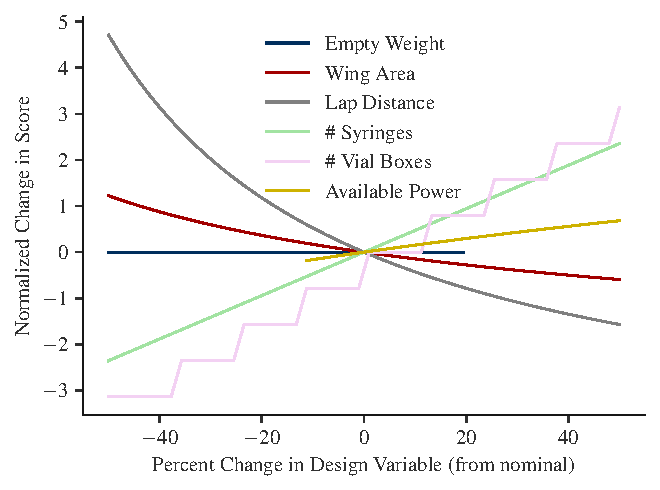
\includegraphics[width=3in]{sensitivityobj}
	}
	\caption{This plot shows the effects of those design parameters that directly affect the increase/decrease in mission scoring beyond simple completion. Lines that do not extend the full range are due to physical impossibilities.}
	\label{fig:sensitivity}
\end{wrapfigure}
Our manufacturing flow follows the outline found in \cref{fig:plannedtiming} which includes three DBF phases.  \Cref{fig:manufacturingplan} shows this flow with more clarity.  Note that for all phases, we will commence CAD roughly a week after design starts, and prototyping a week after that.

\subsubsection{Phase 1} We have completed our conceptual design along with conceptual CAD (see \cref{fig:render}), from which we have built concept prototypes. Foam has dominated our airframe construction in this conceptual prototyping phase as it is cheap and easy to work with using hot-wire, laser-cutter, and hand tools.  We have also built mock vial containers using basic woodworking power tools, as well as simple payload management prototypes using both foam and laser-cut plywood.

\subsubsection{Phase 2} We are currently beginning our preliminary design and CAD from which we will build preliminary prototypes for testing. At this stage, we will continue to use hot-wire cut foam wings/tails with tape hinges for our prototypes, and begin to employ 3D-printed plastic and laser-cut plywood/balsa components for our fuselage and payload manager.  We will use prefabricated composite tubes for tail booms, and use 3D-printed attachment hardware for the various components.

\subsubsection{Phase 3} In January, we will start on our detailed design and CAD, which will lead to our final testing prototypes.  After polishing the design and CAD after final testing, we will manufacture our final competition aircraft. We anticipate utilizing a combination of foam-core, composite wings and tails with live, aramid fiber hinges, 3D-printed plastic and laser cut balsa for the payload manager system components, prefabricated composite tubes for tail booms, and 3D-printed fittings for motor and tail attachments.



%%%%%%%%%%%%%%%%%%%%%%%%%%%%%%%%
%%%% - Critical Processes - %%%%
%%%%%%%%%%%%%%%%%%%%%%%%%%%%%%%%
\subsection{Critical Processes}
\label{ssec:CriticalProcesses}

The most critical processes this year revolve around composite manufacturing methods.  Historically, there has been little to no aircraft production using composites in the BYU Aeronautics Club.  Although there are many other materials and methods that can be used for successful designs, we seek to increase the knowledge base and hands on experience of the members of our team and club.  Therefore, during phase 2, a subset of our team will need to learn, prototype, and teach various composite manufacturing methods to the other members of our team.  We hope to utilize wet layup vacuum bagging techniques for our wing and tail surfaces.  Pending further investigation and testing, we may also include a molded, composite fuselage outer shell, requiring the addition of CNC milling to our critical processes.  In the mean time, our intermediate critical processes include hot-wire foam cutting, 3D printing, and laser-cutting, all of which our team members are familiar with.
